\documentclass[runningheads,a4paper]{llncs}
\usepackage{makeidx}
\usepackage{makecell}
\usepackage{booktabs}
\usepackage{mathtools}
\usepackage{footnote}
\usepackage{nccmath}
\usepackage{amsmath}
\usepackage{amsfonts}
% \usepackage{amssymb}
% \usepackage{amsthm}
\usepackage[utf8]{inputenc}
\usepackage{acronym}
\usepackage{geometry}
\usepackage[hidelinks]{hyperref}
% \hypersetup{pdftex,colorlinks=true,allcolors=blue
\usepackage{float}
\usepackage{graphicx}
\usepackage{cite}
\usepackage{verbatimbox}
% \usepackage{natbib}
\graphicspath{ {Figures/}{imgs/} }
\begin{document}

\frontmatter

\title{MinCall --- MinION end2end convolutional deep learning basecaller}
\author{Neven Miculinić \and Marko Ratković \and Mile Sikić\\
\texttt{\{neven.miculinic, marko.ratkovic, mile.sikic\}@fer.hr}}

\institute{Faculty of
Electrical Engineering and Computing (FER), Zagreb, Croatia}
\maketitle
% \tableofcontents

\begin{abstract}
    The Oxford Nanopore Technologies's MinION is the first portable DNA sequencing device. It's capable of producing long reads, over 100 kBp were reported, however, it has significantly higher error rate than other methods.

    In this study, we created MinCall, an end2end basecaller model for the MinION. The model is based on deep learning and uses convolutional neural networks (CNN) in its implementation. For extra performances is uses cutting edge deep learning techniques and architectures, batch normalization and Connectionist Temporal Classification (CTC) loss.

    The best performing deep learning model achieves state-of-the-art  91.4\% median match rate on E.Coli dataset using R9 pore chemistry and 1D reads.
\keywords{Basecaller, MinION, R9, CNN, CTC, Next generation sequecing}
\end{abstract}

\section{Introduction}
In recent years, deep learning methods significantly improved the state-of-the-art in multiple domains such as computer vision, speech recognition, and natural language processing \cite{LeCun:1998:CNI:303568.303704}\cite{NIPS2012_4824}.
In this paper, we present application of deep learning in the field of  Bioinformatics for DNA basecalling problem.

Oxford Nanopore Technology's MinION nanopore sequencing platform~\cite{mikheyev2014first} is the first portable DNA sequencing device. It's small weight, of only 90 grams, low capital cost, and long read length combined with high-throughput, real-time data analysis, and decent accuracy yield promising results in various applications. From clinical application such as monitoring infectious disease outbreaks~\cite{judge2015early}\cite{quick2016real}, characterizing structural variants in cancer\cite{norris2016nanopore} and even full human genome assembly~\cite{jain2017nanopore}.

Although MinION is able to produce long reads, even up to 882 kb~\cite{loman1-100k,loman2-800k}, they have a high sequencing error rate. This has been somewhat alleviated with new R9 pore model, replacing older R7 ones. In this paper, we show that this error rate can be reduced by our approach with the properly trained neural network model.

The exact error rate metric is unreliable since multiple pipeline tools could be the issue. First the sample is prepared, hopefully, uncontaminated and matching reference genome as close as possible then sequenced using the MinION device obtaining raw data. Next, our model (or any other) comes along and basecalls the sequences. To evaluate error rate metric basecalled read is aligned to the reference genome using aligners with their own errors/biases, most commonly used BWA-MEM~\cite{li2013aligning} and Graphmap~\cite{sovic2016fast}.

\subsection{Sequencing overview}
Conceptually, the MinION sequencer works as follows. It's a variation on now standard shotgun sequencing approach. First, DNA is sheared into smaller DNA fragments and adapters are ligated to either end of the fragments. The resulting DNA fragments pass through a protein embedded in a membrane via a nanometre-sized channel, a nanopore. A single DNA strand passes through the pore. Optionally, hairpin protein adapter can merge two DNA strands, allowing both template and complement read passing through the nanopore sequentially for more accurate reads. This technique is referred as 2D reads, while we focus on 1D reads containing only template DNA and no hairpin adapter.

As DNA strand passes through the nanopore, they are propelled by the current. However, this current varies depending on specific nucleotide context within the nanopore, changing its resistance. We sample the currency multiple times per second, 4000Hz in our dataset, and from this data, we deduce passing DNA fragment. By design, the nanopore is 6 nucleotides wide, and many models use this information internally, yet we opted ours of it in hopes of a simpler model, less feature engineering, and better homopolymer detection.


% \begin{figure}[!ht]
%     \begin{center}
%         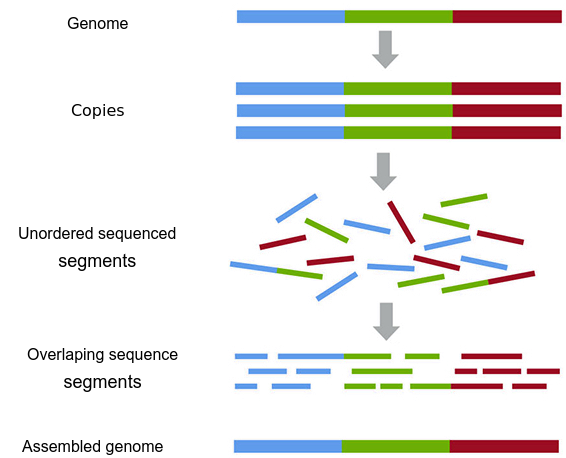
\includegraphics[width=0.6\textwidth]{./imgs/sequencing.png}
%         \caption{Depiction of shotgun sequencing}
%         \label{fg:sequencing}
%     \end{center}
% \end{figure}

\begin{figure}[!ht]
    \begin{center}
        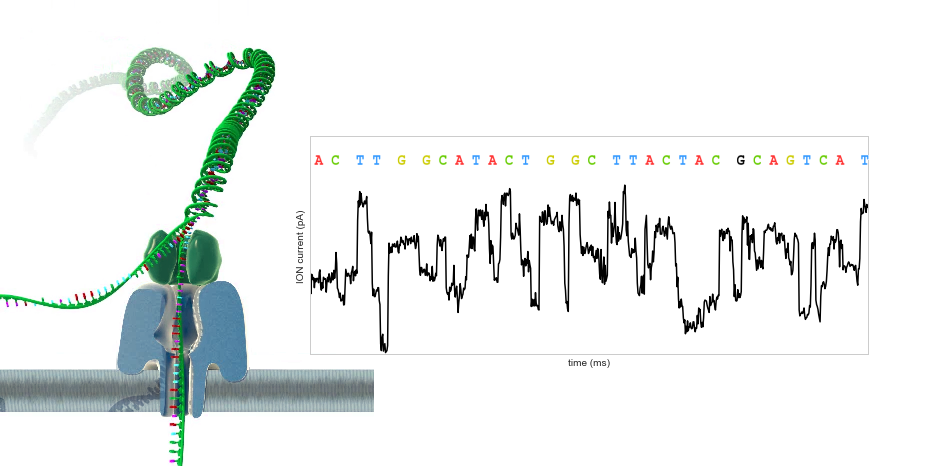
\includegraphics[width=0.7\textwidth]{./imgs/nanopore.png}
        \caption[DNA strain being pulled through a nanopore]{DNA strain being pulled through a nanopore \protect\footnotemark}
        \label{fg:nanopore}
    \end{center}
\end{figure}
\footnotetext{Figure adapted from https://nanoporetech.com/how-it-works}

\section{Related work}
The core of the decoding process is the basecalling step, that is translating the current samples to the nucleotide sequence. Nowadays there are multiple basecalling options, what official and unofficial ones.

Earlier models were Hidden Markov model (HMM)-based where hidden state modeled DNA sequence of length 6 (6-mer) in the nanopore. Pore models were used in computing emission probabilities.~\cite{loman2015complete,schreiber2015analysis,szalay2015novo,timp2012dna} and the recent open source HMM-based basecaller Nanocall~\cite{david2016nanocall}. Modern basecallers use RNN base models, and we opted out using CNN instead with beam search.

We compared our model on R9 chemistry with Metrichor (HMM-based approach), Nanonet\footnote{\url{https://github.com/nanoporetech/nanonet/}} and DeepNano~\cite{deepnano} (RNN based approaches). For the detailed basecaller overview see the appendix~\ref{app:basecallers}.


\section{Dataset}

Dataset used were E.Coli K-12 strands from~\cite{loman1-100k} and Lamba basecalling\footnote{Acquired from doc. dr. sc. Petra Korać and dr.sc. Paula Dobrinić}. Both used datasets show in table \ref{tbl:datasets} have been previously passed through MinKNOW and had been basecalled by Metrichor. As 1D read analysis was the focus of this paper, only those reads were used.

\begin{savenotes}
    \begin{table}[htb]
        \caption{Used datasets}
        \label{tbl:datasets}
        \centering

        \begin{tabular}{lcc| c}
            \toprule
            {} &  \thead{Number of reads} &   \thead{Total bases \lbrack bp\rbrack\footnote{Total number of bases calle by Metrichor}} &    \thead{Whole genome size \lbrack bp\rbrack} \\
            \midrule
            \emph{{E. Coli}}\footnote{R9 sequencing data from \url{http://lab.loman.net/2016/07/30/nanopore-r9-data-release/}, reference taken from \url{https://www.ncbi.nlm.nih.gov/nuccore/48994873}} & 164471 & 1 481 687 490 & 4 639 675\\
            \emph{lambda}\footnote{Internal dataset acquired from doc.~dr.sc.~Petra Korać and dr.sc.~Paula Dobrinić, reference taken from \url{https://www.ncbi.nlm.nih.gov/nuccore/NC_001416.1}}   & 86 &  466 465 & 48 502  \\
            \bottomrule
        \end{tabular}
    \end{table}
\end{savenotes}

\subsection{Data preprocessing}

To help training process, the raw signal is split into smaller blocks that are used as inputs. For each Metrichor basecalled event is easy to determine the block it falls into using \emph{start} field. Using this information output given by Metrichor can be determined for each block.
To correct errors produced by Metrichor and possibly increase the quality of data, each read is aligned to the reference. This is done using aligner GraphMap~\cite{sovic2016fast} that returns the best position in the genome, hopefully, the part of the genome from which read came from.
Alignment part in the genome is used as a target. Using CIGAR string returned by aligner we can correct Metrichor data and get target output for each block. This process is shown in figure~\ref{fg:data_correction}.

\begin{figure}[!ht]
    \begin{center}
        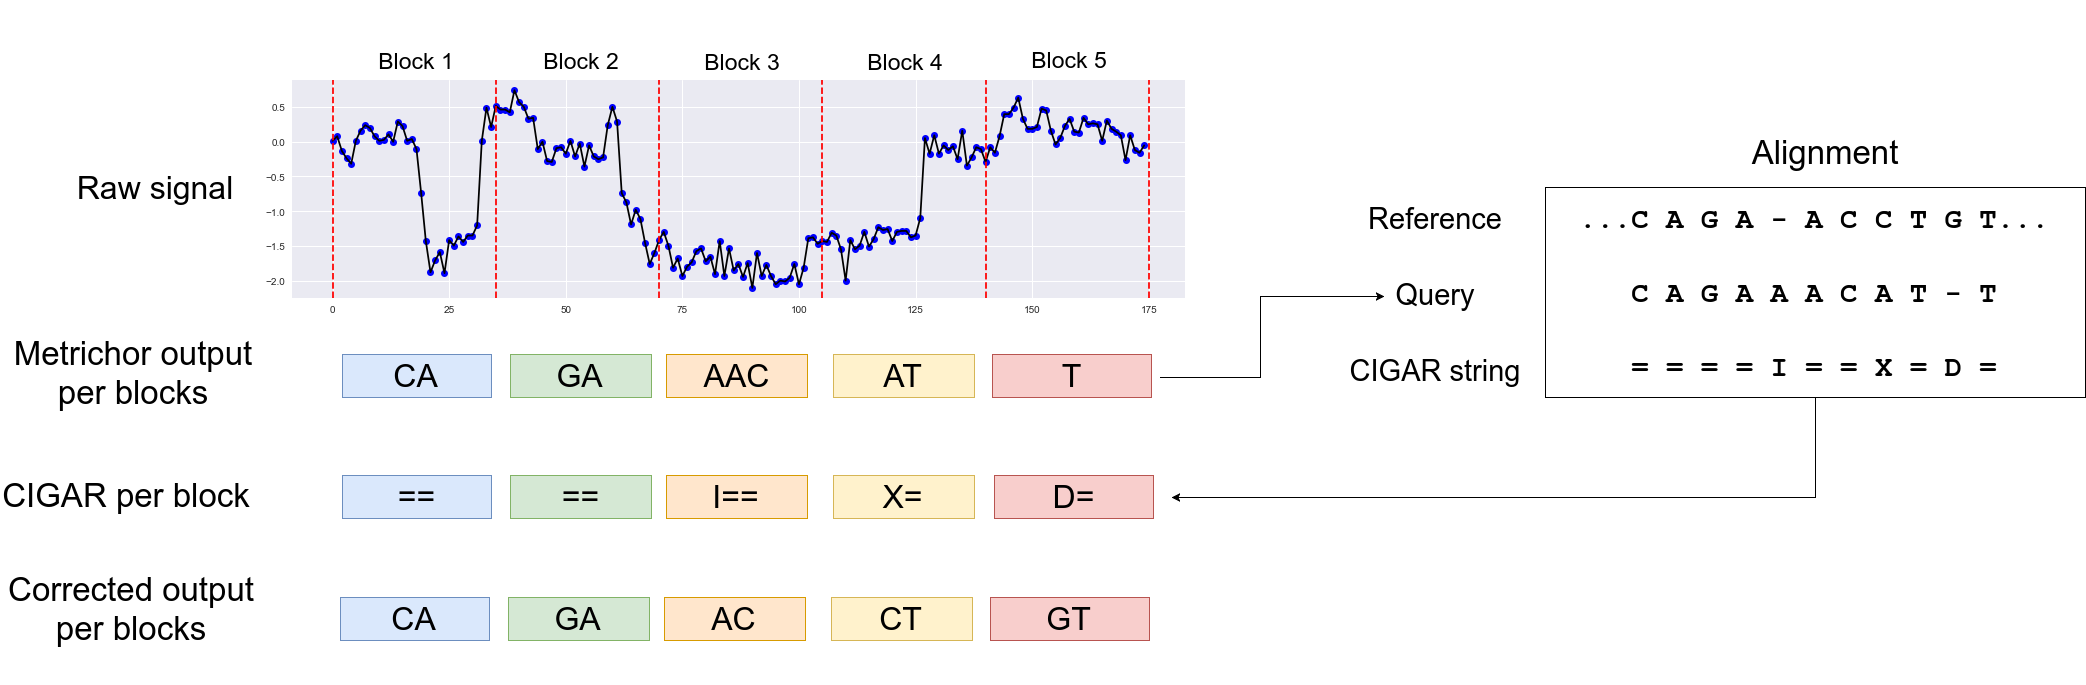
\includegraphics[width=1\textwidth]{./imgs/train_data_correction.png}
        \caption{Dataset preparation}
        \label{fg:data_correction}
    \end{center}
\end{figure}


To eliminate the possibility of overfitting to the known reference, the model is trained and tested on reads from different organisms. Due to the limited amount of public available raw nanopore sequence data, E. Coli was \emph{divided} into two regions.
Reads were split into train and test portions, depending on which region of E. Coli they align.
If read aligns inside first 70\% of the E. Coli, it is placed into train set, and if it aligns to the second portion, it is placed into test set. Reads whose alignment overlaps train and test region are not used. Important to note that E. Coli genome, and genomes of the majority of other bacteria, is cyclical, so reads with alignments that wrap over edges are also discarded. Total train set consist of over 110 thousand reads.
Overview of the entire learning pipeline is shown in figure~\ref{fg:train_pipe}.

\begin{figure}[!ht]
    \begin{center}
        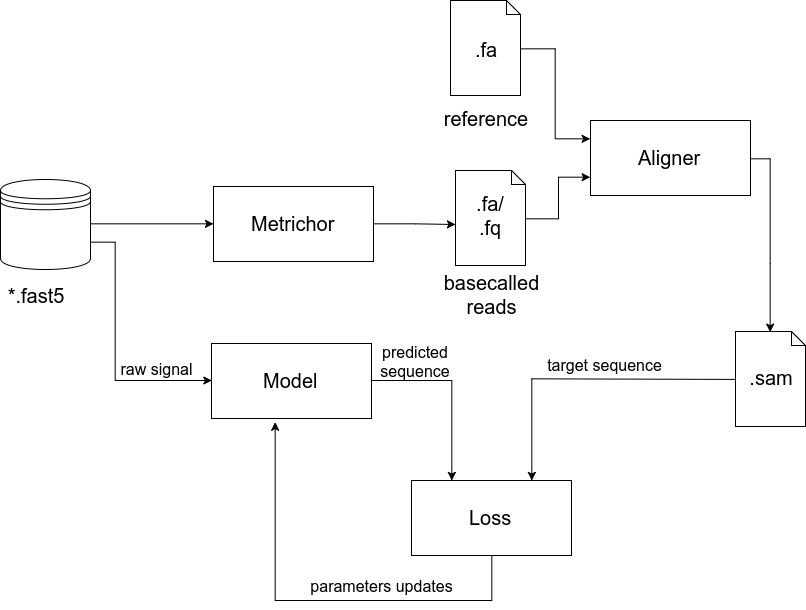
\includegraphics[width=0.7\textwidth]{./imgs/train_pipeline.png}
        \caption{Training pipeline overview}
        \label{fg:train_pipe}
    \end{center}
\end{figure}

\begin{verbbox}
    Target      :  A  G  A  A  A
    Preprocessed:  A  G  A  A' A
\end{verbbox}

\begin{figure}[!h]
    \centering
    \theverbbox
    \caption{Target nucleotide sequence preprocessing}
    \label{fig:data_preprocessing}
\end{figure}

Due to CTC merged nature during decoding, adjacent duplicates are merged into one, we preprocess the target nucleotide sequence with surrogate nucleotides, such that each second repeated nucleotide is replaced with its surrogate. Example provided in figure~\ref{fig:data_preprocessing}. All raw input data were normalized to zero mean and unit variance as it yields superior performance with neural networks.

\section{Method}
Instead of opting for the traditional path using HMM or newly adopted RNN we tried using CNN~(Convolutional neural networks)~\cite{lecun-98}, that is their residual version~\cite{he2016deep}. For loss, we used CTC (Connectionist Temporal Classification)~\cite{graves2006connectionist} between basecalled and the target sequence. Other building blocks used are Batch normalization(BN)~\cite{BNORM} and pooling layers. Dropout~\cite{srivastava2014dropout} was not used.
Described model is implemented using tensorflow~\cite{tensorflow2015-whitepaper} and source warp-ctc~\cite{warpctc} GPU CTC loss implementation.

The final model is a residual neural network consisting of 72 residual blocks BN\footnote{Batch normalization}-ELU\footnote{Exponential Linear Unit

    \begin{equation*}
    \text{ELU}(x)=
    \begin{cases}
    x, & \text{if}\ x>0 \\
    \alpha (exp(x) - 1), & \text{otherwise}
    \end{cases}    \\
    \end{equation*}

}-CONV\footnote{1D convolutional layer}-BN-ELU-CONV, to a grand total of 2 million parameters. The used model is a variant of architecture proposed in paper~\cite{identitet} with the difference of ELU being used as activation instead of ReLU as it is reported \cite{resnet-elu} to speeds up the learning process and improve accuracy as the depth increase.

Each convolutional layer in this models uses 64 channels with kernel size 3. Because sequenced read is always shorter than the raw signal, pooling with kernel size two is used every 24 layers resulting in a reduction of dimensionality by factor 8. This is beneficial in faster learning, better generalization and increased basecalling speed.

Training the model is the minimization of previously described CTC loss. It was done using Adam~\cite{adam} with default parameters, and exponentially decaying learning rate starting from 1e-3 and decay rate of 5e-6 over 100k steps\footnote{We use tf.train.exponential\_decay where current learning rate, lr is $lr=\text{initial\_lr} \cdot \text{decay\_rate}^\frac{\text{global\_step}}{\text{decay\_step}}$} and minibatch size 8. To prevent gradients exploding on bad inputs, they were clipped to a range [-2, 2]. We observed no overfitting due to large dataset size.

During testing, we tried ReLu and PrELU~\cite{prelu} with no significant result difference. We also tried different channel numbers, receptive field width, and various other hyperparameters during hyperparameter optimization and conclude after enough complexity, that is sufficient layers, all choices were performing similarly. We used SigOpt~\cite{dewancker2016strategy}\footnote{\url{https://sigopt.com/}} bayesian hyperparameter optimization library.

\section{Results}

Developed tool was compared with other available basecallers that support R9 chemistry. This includes third-party basically DeepNano and official basecallers by Oxford Nanopore (cloud-based Metrichor and Nanonet).
The fact that ground truth is not known makes evaluation difficult.
Different methods for evaluation were used to get clearer information about each basecaller.

\subsection{Per read metrics}
\label{subs:read_metrics}
A portion of the read length that aligns as correctly is called match\_rate. Same goes for mismatches and insertions.
Sum of all matches, mismatches, and insertions is equal to the reads length \ref{eq:read_len}. For specific details see Appendix~\ref{app:evaluation:CIGAR}. Results on E.Coli test set with Graphmap aligner are shown in table~\ref{tbl:ecoli_rates}. Evaluation with BWM-MEM and on lambda can be found in appendix~\ref{app:evaluation:CIGAR} under tables~\ref{tbl:ecoli_rates_bwa},~\ref{tbl:lambda_rates} and~\ref{tbl:lambda_rates_bwa}. Furthermore we plot Kernel Density estimation(KDE) plots for each mentioned statistic on E.Coli dataset in figure~\ref{fg:ecoli_kde}.

In Appendix~\ref{app:evaluation:CIGAR} the histogram figure~\ref{fg:cigar_op_dist} shows how matches, mismatches, insertions, and deletions are distributed across the reads. It is shown that mismatches and insertion occur more frequently at the beginnings and the ends of the reads. This is not only the case for the developed basecaller, but all other shows the same property. This could be due to lack of context information from both sides when edges are basecalled.

\begin{table}[]
    \caption{Alignment specifications of E. Coli R9 basecalled reads using GraphMap}
    \label{tbl:ecoli_rates}
    \centering
    \begin{tabular}{lcccc}
        \toprule
        {} &  \thead{Match \% \\(median)} &  \thead{Mismatch \% \\(median)} &  \thead{Insertion \% \\(median)} &  \thead{Deletion \% \\(median)} \\
        \midrule
        DeepNano   &                  90.254762 &                      6.452852 &                       \textbf{3.274420} &                     11.829965 \\
        Metrichor  &                  90.560455 &                      5.688105 &                       3.660381 &                      8.328271 \\
        Nanonet    &                  90.607674 &                      5.608912 &                       3.652791 &                      8.299046 \\
        MinCall    &                  \textbf{91.408591} &                     \textbf{ 5.019141} &                       3.477739 &                      \textbf{7.471608 }\\
        \bottomrule
    \end{tabular}
\end{table}

\begin{figure}[]
    \begin{center}
        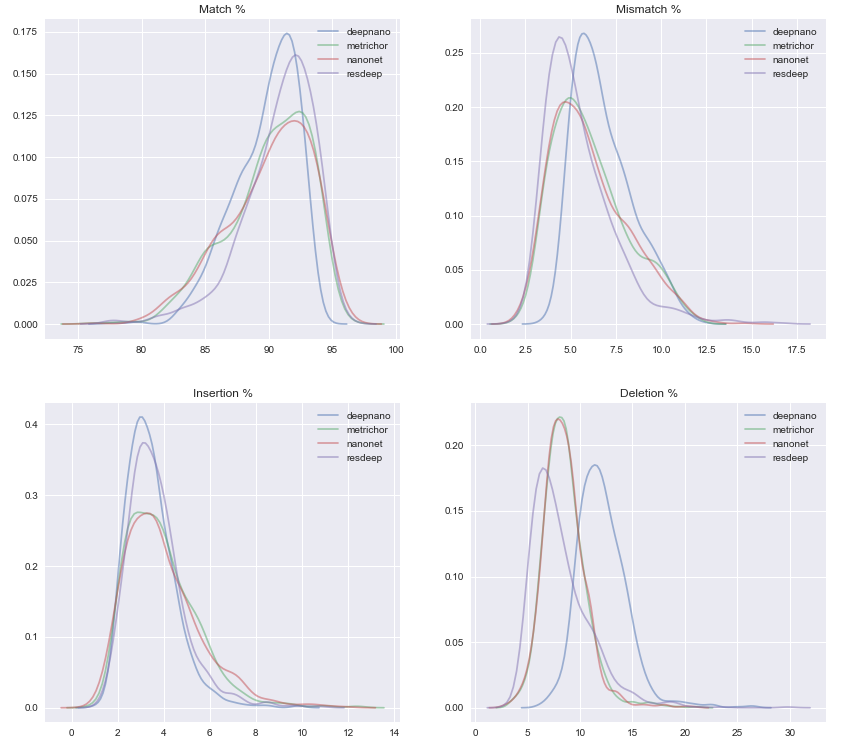
\includegraphics[width=0.8\textwidth]{./imgs/results/ecoli/kde_cigar.png}
        \caption{KDE plot for distribution of percentage of alimnment operations for E. Coli}
        \label{fg:ecoli_kde}
    \end{center}
\end{figure}


\subsection{Consensus metrics}

In Subsection~\ref{subs:read_metrics} we showed metrics after the read is aligned to reference genome. However, if basecalled simply yield nucleotide sequence \emph{A} irrespective of ground truth, it shall have 100\% match rate since it will definitely align somewhere. Therefore we reconstruct the original genome from basecalled reads. Specific metrics definitions analysed are in Appendix~\ref{app:evaluation:consensus}.

\subsubsection{Consensus from pileup}

Instead of going through the whole assembly process, as we know the reference genome of the data used in these tests, we simply align all the reads to the genome, stack them on top of each other forming pileup of read bases. Using majority vote, dominant bases are called on each position. The resulting sequence is called consensus. When calling consensus for deletions,  there has to be a majority of deletions of the same length. Calling insertions has the additional condition, the majority has to agree on both length and the bases of insertion. Figure~\ref{fg:consensus} shows how consensus is called from pileup created from aligned reads. Pileup is stored in mpileup format.

All models show a slight bias towards deletions than insertions, but this may be the limitation of technology as it has been reported that deletion and mismatch rates for nanopore data are ordinarily higher than insertion rates~\cite{sovic2016fast}. Results are shown in table~\ref{tbl:spec_ecoli}. Lambda table is deferred to Appendix in table~\ref{tbl:spec_lambda}.

\begin{figure}[]
   \begin{center}
       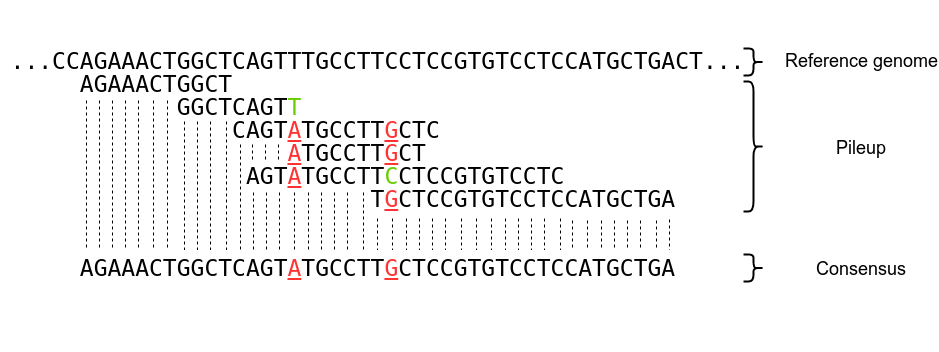
\includegraphics[width=0.8\textwidth]{./imgs/consnesus.png}
       \caption{Consensus from pileup}
       \label{fg:consensus}
   \end{center}
\end{figure}

\begin{table}[]
    \caption{Consensus specifications of E. Coli R9 basecalled reads}
    \label{tbl:spec_ecoli}
    \centering
    \begin{tabular}{lcccccc}
        \toprule
        {} &  \thead{Total called\\\lbrack bp\rbrack} &  \thead{Correctly called\\\lbrack bp\rbrack} &  \thead{Match\\\%} &  \thead{Snp\\\%} &  \thead{Insertion\\\%} &  \thead{Deletion\\\%} \\
        \midrule
        DeepNano  &                  1510244.0 &                      1493242.0 &          98.8742 &         1.0044 &               0.1214 &              0.9041 \\
        Metrichor &                  1515893.0 &                      1502588.0 &          99.1223 &         0.7464 &               0.1313 &              0.6300 \\
        Nanonet   &                  1414237.0 &                      1385515.0 &          97.9691 &         1.5700 &               0.4609 &              1.5158 \\
        resdeep   &                  1517828.0 &                      1506233.0 &          \textbf{99.2361} &         \textbf{0.6474} &               \textbf{0.1165} &             \textbf{ 0.5510 }\\
        \bottomrule
    \end{tabular}
\end{table}


\subsubsection{Consensus from de novo assembly}

In this evaluation method, the consensus sequence is not calculated from the pileup, but by de novo genome assembly. For this task, fast and accurate de novo genome assembler \emph{ra}\footnote{\url{https://github.com/rvaser/ra}}~\cite{vaser} was used and obtained consensus sequence is compared to the reference using dnadiff present in the Mumer\footnote{\url{https://github.com/garviz/MUMmer}}.
The length of the reference, consensus sequence, number of contigs and percentages of aligned bases from the reference to the query and vice versa are shown in the table \ref{tbl:assembly}. Average identity summarizes how closely does the assembled sequence match the reference. This is run on full E. Coli sequence run for 1D template reads (\textasciitilde 160k reads), for both developed tools, Nanonet and Metrichor. Developed tool has shown a small increase in quality of the assembled sequence over Metrichor by offering longer consensus, higher identity percentage, and overall smaller edit distance\footnote{Calculated using \url{https://github.com/isovic/racon/blob/master/scripts/edcontigs.py}}.


\begin{table}[htb]
    \caption{Assembly and consensus results for E. Coli}
    \label{tbl:assembly}
    \centering
\begin{tabular}{lccc}
\toprule
&         Metrichor &           MinCall &          Nanonet \\
\midrule
\thead{Ref. genome size (bp)} &           4639675 &           4639675 &            4639675 \\
\thead{Total bases (bp)}      &           4604806 &           \textbf{4614354} &          4600056 \\
\thead{Contigs [\#]}           &                 1 &                 1 &                1 \\
\thead{Aln. bases ref. (bp)}  &  4639641(100.00\%) &  4639612(100.00\%) &  4639031(99.99\%) \\
\thead{Aln. bases query (bp)} &  4604787(100.00\%) &  4614351(100.00\%) &  4599745(99.99\%) \\
\thead{Avg. Identity}         &             98.76 &             \textbf{99.06} &            98.47 \\
\thead{Edit distance}         &             60418 &             \textbf{46686 }&            74341 \\
\bottomrule
\end{tabular}
\end{table}


\section{Conclusion and further work}

In this paper, we used CNN instead of already tried RNN or HMM approaches, which resulted in in higher accuracy compared to other existing basecallers.
Unlike HMM and RNN, there's no explicit dependency on previous hidden state, therefore this model is massively parallelizable and more sensible given data nature --- that is we're dealing with signal processing, not heavily context-depended language modeling.

All test are done on data for R9 chemistry, but the developed open source code could easily be adjusted and trained on R9.4 and newest R9.5 data when it becomes publicly available.

Currently, without support for newer sequencing data, this model has limited application. It can be used as a demonstration of a different approach to basecalling which yields promising results.  As newer versions of basecallers by Oxford Nanopore do not offer any support for data sequenced with the previous version of chemistries, this tool can be used to re-basecall that data and improvement of the quality of reads retrospectively.

Future work includes experiments with recently proposed Scaled exponential linear units (SELU)~\cite{selu} that eliminate the need for normalization techniques such as used batch normalization. Possible improvements of the model include the combination of convolutions and attention mechanism proposed just recently in the paper~\cite{facebook} showing excellent results in both speed and accuracy, for tasks of language translation. The other option could usage of stacked simple models, such as logistic regression and SVM to predict each nucleotide given raw signal context, similar to our deep learning model pre-CTC layer, and use linear chain CRF for full sequence basecalling.

\section{Acknowledgments}

During this paper creation, we used Sigopt academic license for hyperparameter optimization. We gratefully acknowledge the support of NVIDIA Corporation with the donation of the Titan Xp GPU used for this research.

We're thankful to various other people whose code, tools and advice we've used in completing this project: Fran Jurišić, Ana Marija Selak, Ivan Sović, Robert Vaser and Martin Šošić.

For data, we're thankful for the cooperation of Biologists doc.~dr.~sc. Petra Korać and dr.sc. Paula Dobrinić and Loman labs~\cite{loman1-100k} for publicly posting their dataset.

% set style - not sure which one is official for papers
% spbasic (springer basic makes sense)
% \bibliographystyle{spbasic}
\bibliographystyle{splncs03}
\bibliography{refs}
\appendix
\section{Basecallers}\label{app:basecallers}
Here is currated basecaller list:

\subsection{Official}
\emph{Metrichor} is an Oxford Nanopore company that offers cloud-based platform \emph{EPI2ME} for analysis of nanopore data.
Initially, basecalling was only available by uploading data to the platform - that being the reason why this basecaller is often called Metrichor even though it is a name of the company.

With the release of R9 chemistry, this model was replaced by a more accurate recurrent neural network (RNN) implementation. Currently, Oxford Nanopore offers several RNN-based local basecaller versions under different names: Albacore, Nanonet, and basecaller integrated into MinKNOW \cite{ont-basecallers}.

\emph{Albacore} is basecaller by Oxford Nanopore Technologies ready for production and actively supported.
It is available to the Nanopore Community served as a binary. The source code of Albacore was not provided and is only available through the ONT Developer Channel. The tool supports only R9.4 and future R9.5 version of the chemistry. For R9 tests in this paper, we used R9.4 chemistry setting as instructed on ONT forums.

\emph{Nanonet}\footnote{\url{https://github.com/nanoporetech/nanonet/}} uses the same neural network that is used in Albacore but it is continually under development and does contain features such as error handling or logging needed for production use. It uses the \emph{CURRENNT} library for running neural networks. It supports basecalling of both R9 and R9.4 chemistry versions. However, in our experiments it was painfully slow, which was as expected due to it's classification as not production ready.

\emph{Scrappie}\footnote{\url{https://github.com/nanoporetech/scrappie}} is another basecaller by Oxford Nanopore Technologies. Similar to Nanonet, it is the platform for ongoing development. Scrappie is reported to be the first basecaller  that specifically address homopolymer basecalling. It became publicly available just recently in June 2017 and supports R9.4 and future R9.5 data.

\subsection{Third-party basecallers}
\emph{Nanocall}~\cite{David046086} was the first third-party open source basecaller for nanopore data. It uses HMM approach like the original R7 Metrichor. Nanocall does not support newer chemistries after R7.3.

\emph{DeepNano}~\cite{deepnano}  was the first open-source basecaller based on neural networks. It uses bidirectional recurrent neural networks implemented in Python, using the Theano library. When released, originally only supported R7 chemistry, but support for R9 and R9.4 was added recently.

\section{Evaluation metrics}

\subsection{CIGAR derived metrics}
\label{app:evaluation:CIGAR}

A portion of the read length that aligns as correctly is called match\_rate. Same goes for mismatches and insertions.
Sum of all matches, mismatches, and insertions is equal to the reads length \ref{eq:read_len}.
Here is the specific equation list:

\begin{equation}
\begin{gathered}
\label{eq:read_len}
read\_len =  n\_matches + n\_mismatches + n\_insertions
\end{gathered}
\end{equation}
\begin{equation}
\begin{gathered}
match\_rate = \dfrac{n\_matches}{read\_length}
\end{gathered}
\end{equation}
\begin{equation}
\begin{gathered}
missmatch\_rate = \dfrac{n\_mismatches}{read\_length}
\end{gathered}
\end{equation}
\begin{equation}
\begin{gathered}
insertion\_rate = \dfrac{n\_insertions}{read\_length}
\end{gathered}
\end{equation}

\begin{equation}
\begin{gathered}
match\_rate  + snp\_rate + insertion\_rate = 1
\end{gathered}
\end{equation}

Deletion rate is defined as a total number of deletions in the alignment over the length of the aligned read.

\begin{equation}
\begin{gathered}
deletion\_rate = \dfrac{n\_deletion}{read\_length}
\end{gathered}
\end{equation}


\begin{table}[]
    \caption{Alignment specifications of E. Coli R9 basecalled reads using BWA mem}
    \label{tbl:ecoli_rates_bwa}
    \centering
    \begin{tabular}{lcccc}
        \toprule
        {} &  \thead{Match \% \\(median)} &  \thead{Mismatch \% \\(median)} &  \thead{Insertion \% \\(median)} &  \thead{Deletion \% \\(median)} \\
        \midrule
        DeepNano   &                  90.254762 &                      6.452852 &                       3.274420 &                     11.829965 \\
        Metrichor  &                  90.595441 &                      6.869543 &                       2.531646 &                      7.567381 \\
        Nanonet    &                  90.988989 &                      6.674760 &                     \textbf{  2.348552} &                      7.698530 \\
        MinCall    &                 \textbf{ 91.470588} &                      \textbf{5.929204 }&                       2.477283 &                     \textbf{ 6.970362} \\
        \bottomrule
    \end{tabular}

\end{table}
\begin{table}[]
    \caption{Alignment specifications of Lambda basecalled reads using GraphMap}
    \label{tbl:lambda_rates}
    \centering
    \begin{tabular}{lcccc}
        \toprule
        {} &  \thead{Match \% \\(median)} &  \thead{Mismatch \% \\(median)} &  \thead{Insertion \% \\(median)} &  \thead{Deletion \% \\(median)} \\
        \midrule
        DeepNano   &                  86.997687 &                      9.623494 &                       3.442490 &                     16.052830 \\
        Metrichor  &                  87.714988 &                      7.835052 &                       4.093851 &                     \textbf{10.757491} \\
        Nanonet    &                  88.415611 &                      8.178372 &                       3.629653 &                     11.793022 \\
        MinCall    &                 \textbf{ 89.694482} &                     \textbf{ 7.238095} &                       \textbf{3.078796} &                     13.450292 \\
        \bottomrule
    \end{tabular}

\end{table}
\begin{table}[]
    \caption{Alignment specifications of lambda R9 basecalled reads using BWA mem}
    \label{tbl:lambda_rates_bwa}
    \centering
    \begin{tabular}{lcccc}
        \toprule
        {} &  \thead{Match \% \\(median)} &  \thead{Mismatch \% \\(median)} &  \thead{Insertion \% \\(median)} &  \thead{Deletion \% \\(median)} \\
        \midrule

        DeepNano   &                  86.625973 &                     11.288361 &                       2.098225 &                     14.648308 \\
        Metrichor  &                  87.294093 &                     10.109186 &                       2.376476 &                      \textbf{9.645323 }\\
        Nanonet    &                  87.767037 &                     10.017598 &                       2.354248 &                     10.597232 \\
        MinCall    &                 \textbf{ 89.049870} &                     \textbf{ 9.480883} &                       \textbf{1.615188 }&                     12.962441 \\
        \bottomrule
    \end{tabular}
\end{table}


\begin{figure}[!ht]
    \begin{center}
        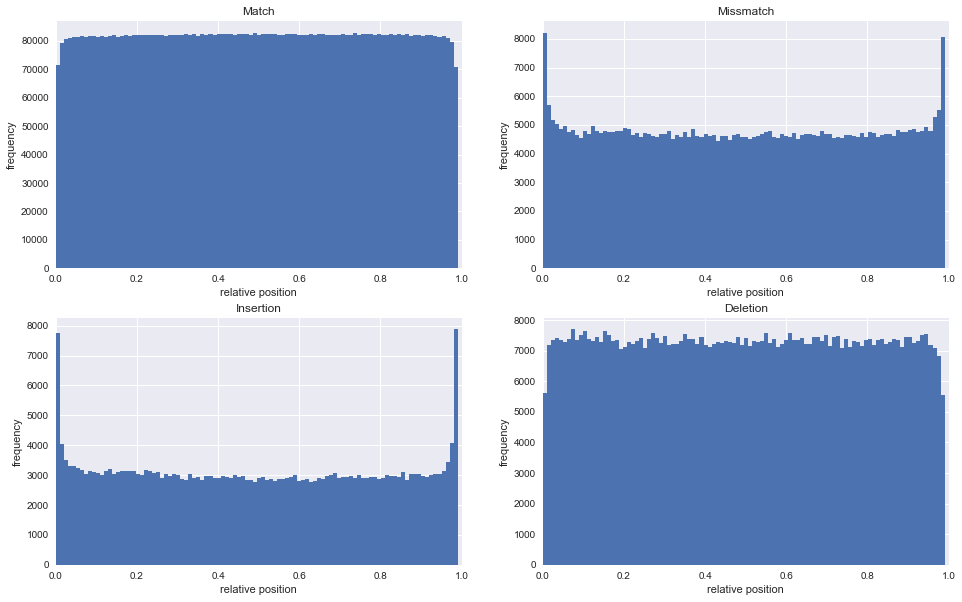
\includegraphics[width=1\textwidth]{./imgs/operation_distributed_r9.png}
        \caption{Histogram of alignment operations over relative position inside of read}
        \label{fg:cigar_op_dist}
    \end{center}
\end{figure}

\subsection{Consensus metrics}
\label{app:evaluation:consensus}

Similarly, as before, match rate, mismatch rate, insertion and deletion rates are calculated but this time for whole consensus sequence. In this context, mismatches are called \emph{single nucleotide polymorphisms} (snp).

\begin{equation}
\begin{gathered}
match\_rate = \dfrac{n\_correct\_bases}{consensus\_length}
\end{gathered}
\end{equation}
\begin{equation}
\begin{gathered}
snp\_rate = \dfrac{n\_snp}{consensus\_length}
\end{gathered}
\end{equation}
\begin{equation}
\begin{gathered}
insertion\_rate = \dfrac{n\_insertions}{consensus\_length}
\end{gathered}
\end{equation}

\begin{equation}
\begin{gathered}
match\_rate  + snp\_rate + insertion\_rate = 1
\end{gathered}
\end{equation}


\begin{equation}
\begin{gathered}
deletion\_rate = \dfrac{n\_deletion}{consensus\_length}
\end{gathered}
\end{equation}

\begin{table}[]
    \caption{Consensus specifications of lambda R9 basecalled reads}
    \label{tbl:spec_lambda}
    \centering
    \begin{tabular}{lcccccc}
        \toprule
        {} &  \thead{Total called\\\lbrack bp\rbrack} &  \thead{Correctly called\\\lbrack bp\rbrack} &  \thead{Match\\\%} &  \thead{Snp\\\%} &  \thead{Insertion\\\%} &  \thead{Deletion\\\%} \\
        \midrule
        DeepNano  &                    48342.0 &                        48025.0 &          99.3443 &         0.6433 &               \textbf{0.0124} &              0.2648 \\
        Metrichor &                    48469.0 &                        48257.0 &          \textbf{99.5626} &         \textbf{0.4188} &               0.0186 &              \textbf{0.1465} \\
        Nanonet   &                    48438.0 &                        48168.0 &          99.4426 &         0.5409 &               0.0165 &              0.1961 \\
        resdeep   &                    48385.0 &                        48163.0 &          99.5412 &         0.4402 &               0.0186 &              0.1976 \\
        \bottomrule
    \end{tabular}
\end{table}


\end{document}
